\chapter{Diagramas de estado}
Los diagramas de estado son una de las herramientas que permiten mostrar como es el comportamiento de los objeto o las variables dentro del programa, esto quiere decir, que permiten registarar como evolucionan lentamente los objetos en tiempo de ejecución.

Estos diagramas tienen dos elementos sobresalientes: los estados y las transiciones.

Los estados son los que indican los distintos cambios que tienen los objetos en el tiempo de ejecución, por otro lado las trancisiones son los eventos que suceden para que un objeto pase de un estado a otro. Las transiciones tienen tres elementos importantes: el disparador, la condición y el efecto.

El disparador es la acción que permite que genera el cambio; la condición, como su nombre lo dice, es el prerequisito que debe solventarse para que se genere e cambio y finalmente el efecto es el resultado que se produce en el objeto para ue pase al siguiente estado.

A continuación mostraremos un aplicación de estos diagramas, aplicandolos en el proyecto Cine+:
\begin{itemize}
\item{Clase Asiento}
\begin{figure}[h!]
	\centering
		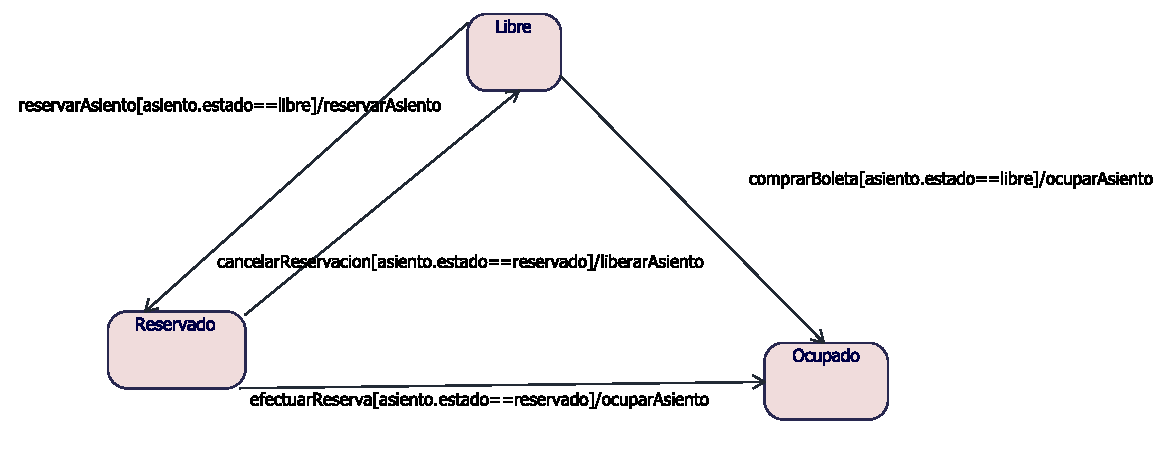
\includegraphics[scale=0.6]{diseno/estado/imgs/estadosAsiento}
	\caption{Diagrama de Estado para la clase Asiento}
\end{figure}

Como se puede ver en la anterior imagen, existen un cambio entre la dispoibilidad de un asiento, pero una vez ocupado nunca puede cambiar de estado. La ventaja de los diagramas de estado es que permite ser incluidos en un diagrama de clases, tal y como se muestra en la siguiente imagen.
\begin{figure}[h!]
	\centering
		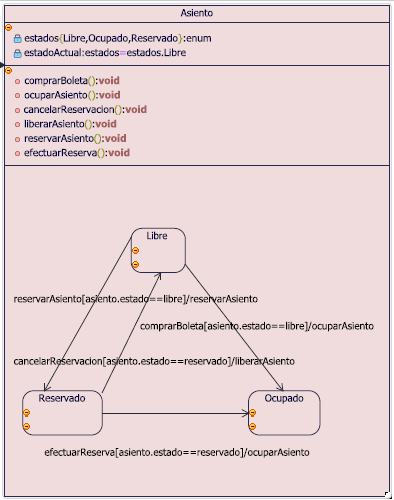
\includegraphics[scale=0.6]{diseno/estado/imgs/estadoClaseAsiento}
	\caption{Clase Asiento}
\end{figure}

Una clase que contiene todas estas carecterísticas no es un diseño que sea correcto, esto se debe que en caso de que se tenga que agregar una nueva clase de disponibilidad se entrará en el problema de modificar toda la clase. Para evitar esta dificultad se puede utilizar un patron GoF de diseño, en este caso se usará el patrón estado, el cual da la posibilidad de extender las necesidades que puedan llegar a tenerse. 

\begin{figure}[h!]
	\centering
		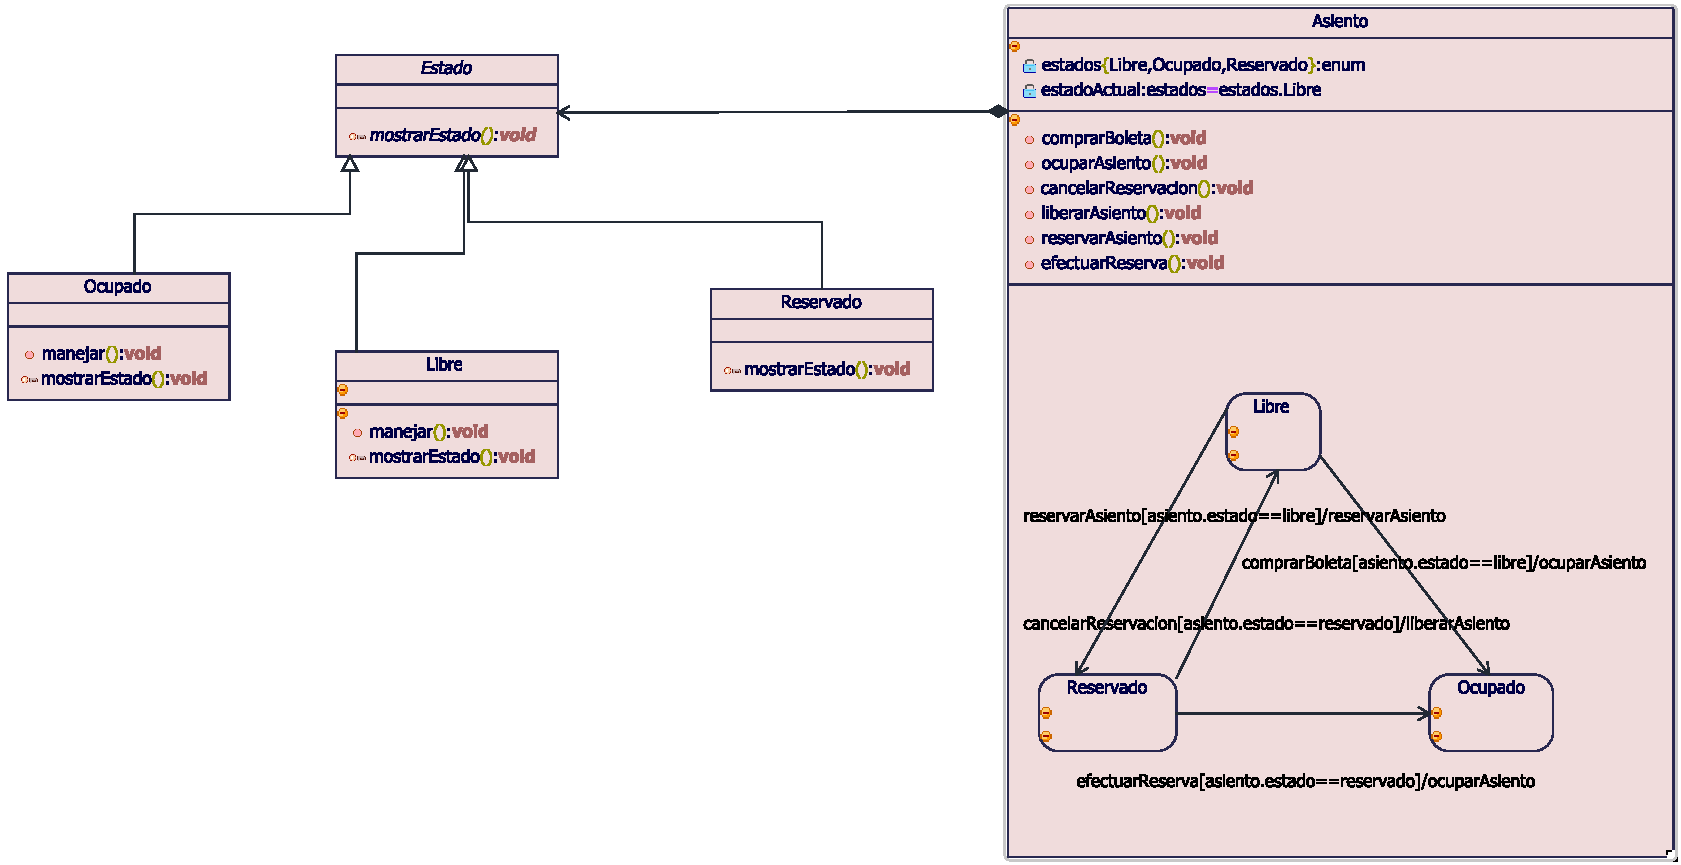
\includegraphics[scale=0.6]{diseno/estado/imgs/patronEstadoAsiento}
	\caption{Patrón Estado para la clase Asiento}
\end{figure}
\item{Clase Reserva}
\begin{figure}[h!]
	\centering
		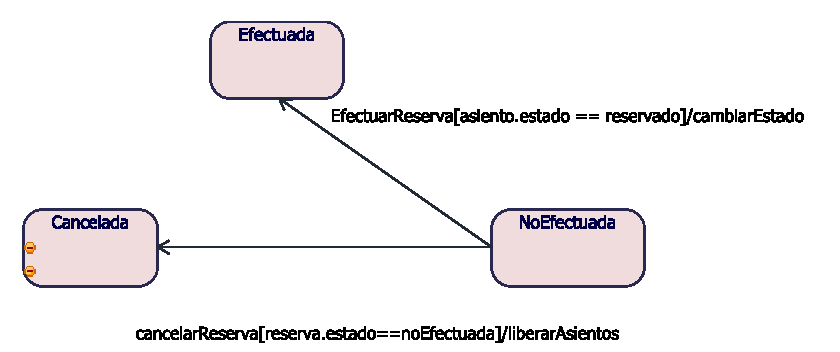
\includegraphics[scale=0.8]{diseno/estado/imgs/estadosReserva}
	\caption{Diagrama de estados para la clase Reserva}
\end{figure}
\begin{figure}[H]
	\centering
		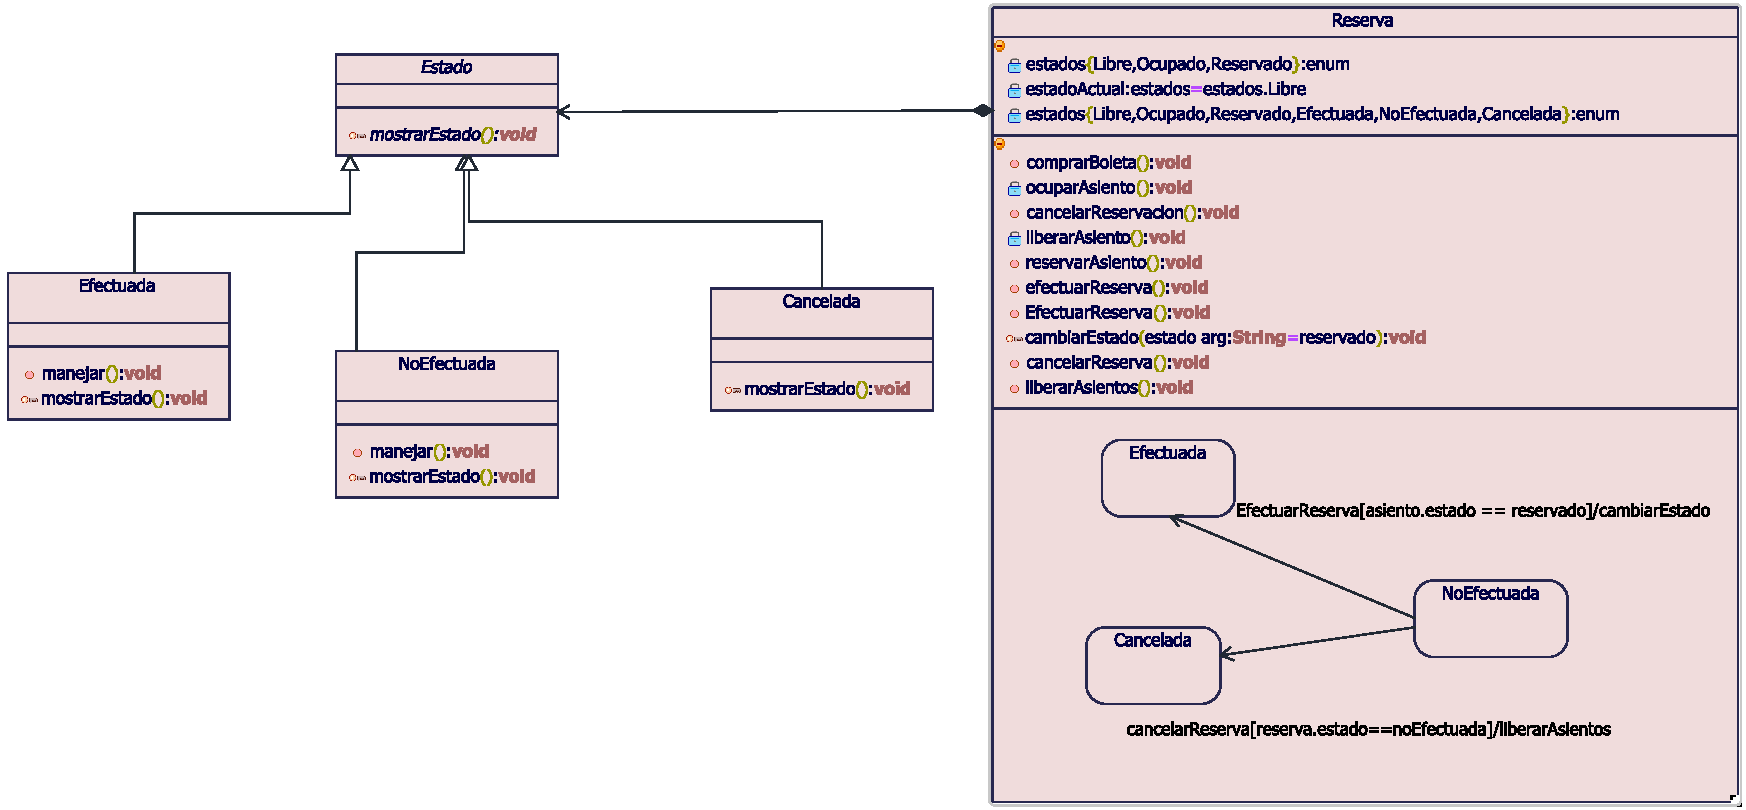
\includegraphics[scale=0.6]{diseno/estado/imgs/patronEstadoReserva}
	\caption{Patrón Estado para la clase Reserva}
\end{figure}
\end{itemize}
